\documentclass{article}
\usepackage{amsmath, amssymb, tikz, multicol}
\usepackage{xcolor, colortbl} % colour-related things
\usepackage{longtable} % long tabular environment
\usepackage{tcolorbox}
\usepackage{enumitem}
\usepackage{hhline}
\usepackage{algpseudocode, algorithm}

\usepackage{geometry}
\geometry{
   a4paper,
   total={170mm,257mm},
   left=30mm,
   right=30mm,
   top=30mm,
   bottom=30mm
}

\newtcolorbox{coolbox}[1]{
   colframe=black!75!white, 
   colback=black!10!white,
   boxrule=1pt,
   halign=flush left,
   sharp corners, 
   title = {\centering\textbf{\textrm{#1}}},
   arc = 0.001mm, % fixes display problems with some pdf viewers
   subtitle style = {
      boxrule=1pt,
      colback=black!50!white,
   }
}

\renewcommand{\L}{\mathcal{L}}

\begin{document}
\begin{flushleft}
   \begin{center}
      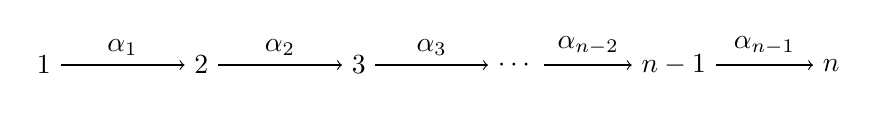
\begin{tikzpicture}
         \node (A) at (0,0) {1};
         \node (B) at (2,0) {2};
         \node (C) at (4,0) {3};
         \node (D) at (6,0) {$\cdots$};
         \node (E) at (8,0) {$n-1$};
         \node (F) at (10,0) {$n$};
         \draw[->] (A) -- (B) node[midway, anchor=south] {$\alpha_1$};
         \draw[->] (B) -- (C) node[midway, anchor=south] {$\alpha_2$};
         \draw[->] (C) -- (D) node[midway, anchor=south] {$\alpha_3$};
         \draw[->] (D) -- (E) node[midway, anchor=south] {$\alpha_{n-2}$};
         \draw[->] (E) -- (F) node[midway, anchor=south] {$\alpha_{n-1}$};
      \end{tikzpicture}
   \end{center}

   \subsection*{What are we doing?}
   Given a type $A$ Dynkin quiver $Q$ with $n \geq 3$ vertices and a finite set of relations on $Q$, 
   we form the quotient algebra $kQ/I$, where $kQ$ is the path algebra of $Q$ over the rationals and $I$ 
   is the principal ideal generated by the relations. \\[\baselineskip]

   Our goal is to investigate whether $kQ/I$ is fractional Calabi-Yau (FCY) or not for a variety of different relations.
   To do so, we have a few different algorithms, which will be detailed immediately. \\[\baselineskip]

   \begin{coolbox}{\texttt{v1} (Version 1)}
      This algorithm works as follows:
      \begin{enumerate}[label=\textbf{(\roman*)}]
         \item Determines the trivial extension algebra $T$ of $kQ/I$.
         \item Determines $M$, which is defined to be $T$ as a right-module over the enveloping algebra of $T$.
         \item Checks whether $M$ is $\Omega$-periodic. This is done by checking whether $\Omega^i\left(M\right) \cong M$
            for all $1 \leq i \leq N$, where $N > 0$ is provided. If such an $i$ exists, then it is returned and the algorithm
            terminates. Otherwise, we return ``\texttt{maximum syzygy exceeded}" and the algorithm terminates. 
      \end{enumerate}
   \end{coolbox}

   \begin{coolbox}{\texttt{v2} (Version 2)}
      This algorithm works as follows:
      \begin{enumerate}[label=\textbf{(\roman*)}]
         \item Determines the trivial extension algebra $T$ of $kQ/I$.
         \item Determines the set of all simple modules $S$ of $T$.
         \item Calculates the direct sum $\mathcal{D} = \displaystyle \bigoplus_{s \in S} s.$
         \item Checks whether $\mathcal{D}$ is $\Omega$-periodic. This is done by checking whether 
            $\Omega^i\left(\mathcal{D}\right) \cong \mathcal{D}$
            for all $1 \leq i \leq N$, where $N > 0$ is provided. If such an $i$ exists, then it is returned and the algorithm
            terminates. Otherwise, we return ``\texttt{maximum syzygy exceeded}" and the algorithm terminates. 
      \end{enumerate}
   \end{coolbox}

   \begin{coolbox}{\texttt{v3} (Version 3)}
      This algorithm works as follows:
      \begin{enumerate}[label=\textbf{(\roman*)}]
         \item Determines the trivial extension algebra $T$ of $kQ/I$.
         \item Determines the set of all simple modules $S$ of $T$.
         \item Checks whether each $\sigma \in S$ is $\Omega$-periodic. This is done by checking whether 
            $\Omega^i\left(\sigma \right) \cong \sigma$
            for all $1 \leq i \leq N$, where $N > 0$ is provided. If such an $i$ exists, then it is returned and the algorithm
            terminates. Otherwise, we return ``\texttt{maximum syzygy exceeded}" and the algorithm terminates. 
      \end{enumerate}
   \end{coolbox}

   \newpage

   \section{Results}
   Below, we present the results for different values of $n$. For convenient abbreviation, we use the notation $\ell_k$ to refer to all principal 
   ideals generated by any (finite) number of length $k$ relations. Table rows are highlighted in {\color{red!50!white}\textbf{red}} whenever we have an ideal
   that might have the potential for $kQ/I$ to not be FCY.
   \begin{center}
      $n=3$
      \begin{longtable}{|c|c|c|c|}
         \hline
         $I$ & \texttt{v1} & \texttt{v2} & \texttt{v3} \\
         \hline 
         () & 6 & & 6 \\
         \hline
         $(a_1a_2)$ & 6 & & 6\\
         \hline
      \end{longtable}

      $n=4$

      \begin{longtable}{|c|c|c|c|}
         \hline 
         $I$ & \texttt{v1} & \texttt{v2} & \texttt{v3} \\
         \hline 
         $()$ & 8 && 8 \\
         \hhline{|=|=|=|=|}
         $(a_1a_2)$ & 8 & & 8\\
         $(a_2a_3)$ & 8 && 8\\
         $(a_1a_2, a_2a_3)$ & 8 && 8\\
         \hhline{|=|=|=|=|}
         $(a_1a_2a_3)$ & 10 && 5\\
         \hline
      \end{longtable}

      $n=4$ (mixed relations)

      \begin{longtable}{|c|c|c|c|}
         \hline 
         $I$ & \texttt{v1} & \texttt{v2} & \texttt{v3} \\
         \hline
         $(a_1a_2, a_1a_2a_3)$ & 8 & & 8\\
         $(a_2a_3, a_1a_2a_3)$ & 8 & & 8\\
         $(a_1a_2, a_2a_3, a_1a_2a_3)$ & 8 & & 8\\
         \hline
      \end{longtable}

      $n=5$
      \begin{longtable}{|c|c|c|c|}
         \hline
         $I$ & \texttt{v1} & \texttt{v2} & \texttt{v3} \\
         \hline
         $()$ & 10 && 10 \\
         \hhline{|=|=|=|=|}
         $(a_1a_2)$ & 10 && 10\\
         $(a_2a_3)$ & 10 && 10 \\
         $(a_3a_4)$ & 10 && 10\\
         $(a_1a_2, a_2a_3)$ & 10 && 10 \\
         $(a_1a_2, a_3a_4)$ & 10 && 10 \\
         $(a_1a_2, a_2a_3, a_3a_4)$ & 10 && 10 \\
         \hhline{|=|=|=|=|}
         $(a_1a_2a_3)$ & 14 && 14\\
         $(a_2a_3a_4)$ & 14 && 14\\
         $(a_1a_2a_3, a_2a_3a_4)$ & 14 && 14\\
         \hhline{|=|=|=|=|}
         $(a_1a_2a_3a_4)$ & 14 && 14\\
         \hline
      \end{longtable}

      $n=5$ (mixed relations)
      \begin{longtable}{|c|c|c|c|}
         \hline
         $I$ & \texttt{v1} & \texttt{v2} & \texttt{v3} \\
         \hline
         $(a_1a_2,a_1a_2a_3)$ &&& 10 \\
         $(a_1a_2,a_2a_3a_4)$ &&& 14 \\
         $(a_1a_2,a_1a_2a_3,a_2a_3a_4)$ &&& 14 \\
         %%%
         $(a_2a_3,a_1a_2a_3)$ &&& 10 \\
         $(a_2a_3,a_2a_3a_4)$ &&& 10 \\
         $(a_2a_3,a_1a_2a_3,a_2a_3a_4)$ &&& 10 \\
         %%%
         $(a_1a_2,a_2a_3,a_1a_2a_3)$ &&& 10 \\
         $(a_1a_2,a_2a_3,a_2a_3a_4)$ &&& 10 \\
         $(a_1a_2,a_2a_3,a_1a_2a_3,a_2a_3a_4)$ &&& 10 \\
         %%%
         $(a_3a_4,a_1a_2a_3)$ &&& 14 \\
         $(a_3a_4,a_2a_3a_4)$ &&& 10 \\
         $(a_3a_4,a_1a_2a_3,a_2a_3a_4)$ &&& 14 \\
         %%%
         $(a_1a_2,a_3a_4,a_1a_2a_3)$ &&& 10 \\
         $(a_1a_2,a_3a_4,a_2a_3a_4)$ &&& 10 \\
         $(a_1a_2,a_3a_4,a_1a_2a_3,a_2a_3a_4)$ &&& 10 \\
         %%%
         $(a_2a_3,a_3a_4,a_1a_2a_3)$ &&& 10 \\
         $(a_1a_2,a_3a_4,a_2a_3a_4)$ &&& 10 \\
         $(a_1a_2,a_3a_4,a_1a_2a_3,a_2a_3a_4)$ &&& 10 \\
         %%%
         $(a_1a_2,a_2a_3,a_3a_4,a_1a_2a_3)$ &&& 10 \\
         $(a_1a_2,a_2a_3,a_3a_4,a_2a_3a_4)$ &&& 10 \\
         $(a_1a_2,a_2a_3,a_3a_4,a_1a_2a_3,a_2a_3a_4)$ &&& 10 \\
         \hline
         $\ell_{2,3}$ &&& 10 \\
         \hline
         $\ell_{3,4}$ &&& 14 \\
         \hline
      \end{longtable}

      $n=6$
      \begin{longtable}{|c|c|c|c|}
         \hline
         $I$ & \texttt{v1} & \texttt{v2} & \texttt{v3} \\
         \hline 
         $()$ & && 12 \\
         \hhline{|=|=|=|=|} 
         $(a_1a_2)$ & 12 && 12 \\
         $(a_2a_3)$ & 12 && 12 \\
         $(a_3a_4)$ & 12 && 12 \\
         $(a_4a_5)$ & 12 && 12 \\
         $(a_1a_2, a_2a_3)$ & 12 && 12 \\
         $(a_1a_2, a_3a_4)$ & 12 && 12 \\
         $(a_1a_2, a_4a_5)$ & 12 && 12 \\
         $(a_2a_3, a_3a_4)$ & 12 && 12 \\
         $(a_2a_3, a_4a_5)$ & 12 && 12 \\
         $(a_3a_4, a_4a_5)$ & 12 && 12 \\
         $(a_1a_2, a_2a_3, a_3a_4)$ & 12 && 12 \\
         $(a_1a_2, a_2a_3, a_4a_5)$ & 12 && 12 \\
         $(a_1a_2, a_3a_4, a_4a_5)$ & 12 && 12 \\
         $(a_2a_3, a_3a_4, a_4a_5)$ & 12 && 12 \\
         $(a_1a_2, a_2a_3, a_3a_4, a_4a_5)$ & 12 && 12 \\
         \hhline{|=|=|=|=|} 
         $(a_1a_2a_3)$ && 9 & 9 \\
         $(a_2a_3a_4)$ && 11 & 22\\
         $(a_3a_4a_5)$ && 9 & 9\\
         $(a_1a_2a_3, a_2a_3a_4)$ && 9 & 9 \\
         \rowcolor{red!50!white}
         $(a_1a_2a_3, a_3a_4a_5)$ && $>30$ & $>50$ \\
         $(a_2a_3a_4, a_3a_4a_5)$ && 9 & 9\\
         $(a_1a_2a_3, a_2a_3a_4, a_3a_4a_5)$ && 22 & 22 \\
         \hhline{|=|=|=|=|} 
         $(a_1a_2a_3a_4)$ && 22 & 22\\
         $(a_2a_3a_4a_5)$ && 22 & 22\\
         $(a_1a_2a_3a_4, a_2a_3a_4a_5)$ && 22 & 22\\
         \hhline{|=|=|=|=|} 
         $(a_1a_2a_3a_4a_5)$ && 9 & 9 \\
         \hline
      \end{longtable}
      
      \newpage

      $n=6$ (mixed relations)
      \begin{longtable}{|c|c|c|c|}
         \hline
         $I$ & \texttt{v1} & \texttt{v2} & \texttt{v3} \\
         \hline 
         $\ell_{2,3}$ &&& 9, 12, 22 \\
         $\ell_{2,4}$ &&& 12, 22 \\
         $\ell_{2,5}$ &&& 12 \\
         $\ell_{3,4}$ \textbf{not} containing $(a_1a_2a_3,a_3a_4a_5)$ &&& 9, 22 \\
         \hline
         \rowcolor{red!50!white}
         $\ell_{3,4}$ containing $(a_1a_2a_3,a_3a_4a_5)$ &&& $>30$ \\
         \hline
         $\ell_{3,5} \setminus \{\xi\}$ &&& 9, 22 \\
         \hline
         \rowcolor{red!50!white}
         $\xi = (a_1a_2a_3,a_3a_4a_5, a_1\ldots a_5)$ &&& $>30$ \\
         \hline
         $\ell_{4,5}$ &&& 22 \\
         \hline
      \end{longtable}

      $n=7$
      \begin{longtable}{|c|c|c|c|}
         \hline
         $I$ & \texttt{v1} & \texttt{v2} & \texttt{v3} \\
         \hline
         $\ell_2$ &&& 14 \\
         \hline
         $(a_1a_2a_3)$ &&& 22 \\
         $(a_2a_3a_4)$ &&& 17 \\
         $(a_3a_4a_5)$ &&& 17 \\
         $(a_1a_2a_3, a_2a_3a_4)$ &&& 22 \\
         \rowcolor{red!50!white}
         $(a_1a_2a_3,a_3a_4a_5)$ &&& $>24$ \\
         \hline
         $(a_1a_2a_3a_4)$ &&& 17 \\
         \rowcolor{red!50!white}
         $(a_2a_3a_4a_5)$ &&& $>50$ \\
         $(a_3a_4a_5a_6)$ &&& 17 \\
         $(a_1a_2a_3a_4, a_2a_3a_4a_5)$ &&& 17 \\
         \rowcolor{red!50!white}
         $(a_1a_2a_3a_4, a_3a_4a_5a_6)$ &&& $>50$ \\
         $(a_2a_3a_4a_5, a_3a_4a_5a_6)$ &&& 17 \\
         $(a_1a_2a_3a_4, a_2a_3a_4a_5, a_3a_4a_5a_6)$ &&& 17 \\
         \hline
         $\ell_5$ &&& 17 \\
         \hline
         $\ell_6$ &&& 17 \\
         \hline
      \end{longtable}

      $n=7$ (mixed relations)

      \begin{longtable}{|c|c|c|c|}
         \hline
         $I$ & \texttt{v1} & \texttt{v2} & \texttt{v3} \\
         \hline
         $\ell_{4,5}$ excluding problematic ideals &&& 17 \\
         \rowcolor{red!50!white}
         $\ell_{4,5}$ with problematic ideals &&& $>30$ \\
         $\ell_{4,6}$ excluding problematic ideals &&& 17 \\
         \rowcolor{red!50!white}
         $\ell_{4,6}$ with problematic ideals &&& $>30$ \\
         $\ell_{5,6}$ &&& 17 \\
         \hline
      \end{longtable}

      $n=8$
      \begin{longtable}{|c|c|c|c|}
         \hline
         $I$ & \texttt{v1} & \texttt{v2} & \texttt{v3} \\
         \hline
         $\ell_2 \setminus \{\lambda\}$ && 16 & 16\\
         $\lambda = (a_1a_2, a_2a_3, a_3a_4, a_4a_5, a_5a_6, a_6a_7)$ && 8 & 16 \\
         $(a_1a_2a_3)$ &&& 13 \\
         $(a_2a_3a_4)$ &&& 29 \\
         \rowcolor{red!50!white}
         $(a_3a_4a_5)$ &&& $>50$ \\
         $(a_4a_5a_6)$ &&&  ?\\
         $(a_5a_6a_7)$ &&&  ?\\
         \hline
      \end{longtable}

      $n = 9$
      \begin{longtable}{|c|c|c|c|}
         \hline
         $I$ & \texttt{v1} & \texttt{v2} & \texttt{v3} \\
         \hline
         $\ell_2$ &&& 18 \\
         \hline
         \rowcolor{red!50!white}
         $(a_1 \ldots a_6)$ &&& $>39$ \\
         \rowcolor{red!50!white}
         $\ell_7$ &&& $>50$ \\
         \hline
         $\ell_8$ &&& 30 \\
         \hline
      \end{longtable}
      
   \end{center}
   \section{A few questions}
   \textbf{Conjecture 1:} Given an ideal $I$, if $kQ_n/I$ is not FCY, then $kQ_N/I$ is not FCY for all $N > n$. \\
   \textbf{Conjecture 2:} If $I \in \ell_2$, then $kQ_n / I$ is FCY for any valid $n$. \\
   \textbf{Conjecture 3:} The dimension of ideals corresponding to length two relations is always $2n$. \\
   \textbf{Conjecture 4:} Given some ideal $I \in \ell_k$, if $kQ/I$ is not FCY, then $kQ/J$ is not FCY, 
   where $J$ is any mixed relation ideal containing $I$.
\end{flushleft}

\begin{algorithm}
   \begin{algorithmic}[1]
      \caption{Determining the projectives and injectives.}
      \Require $R = [(s_1, t_1), (s_2, t_2), \ldots, (s_m, t_m)]$ \Comment{A list of $m$ relations on $Q_n$}.
      \State $P, I \gets \big[[1, \ldots, n],\; [2, \ldots, n],\; \ldots, [n]\big]$ \Comment{These lists store the projectives and injectives.}
      \For{$r \in R$}
      \For{$r[1] \leq v \leq n$} 
      \State Delete every element $1 \leq e \leq r[0]$ from $P[v]$. \Comment{Projectives.}
      \EndFor

      \For{$1 \leq v \leq r[0]$} 
      \State Delete every element $r[1] \leq e \leq n$ from $I[v]$. \Comment{Injectives.}
      \EndFor
      \EndFor
   \end{algorithmic}
\end{algorithm}

\subsection*{Kernel of Modules}
Given two modules $M_1 = (\alpha,\beta_1)$ and $M_2 = (\alpha,\beta_2)$, we have that 
\[
   \ker(M_1,M_2) = 
   \begin{cases}
      (0,0), & \text{if } \beta_1 = \beta_2; \\
      \big(\max(\beta_1,\beta_2) - 1, \; \min(\beta_1, \beta_2)\big), & \text{otherwise.}
   \end{cases}
\]
\end{document}
